\chapter{Prédire les interactions biotiques au sein de milieux pauvres en données}
\label{chap3}

\section{Résumé en français du deuxième article}

\subsection{Contexte scientifique}

\subsection{Publication associée}

\subsection{Traduction du résumé de l'article publié}

\section{Title}

Thinking outside the box – predicting biotic interactions in data-poor environments

\section{Authors}

David Beauchesne, Philippe desjardins-proulx2016, Philippe Archambault, Dominique Gravel

% ---------------------------------
% ---------------------------------
%           ABSTRACT
% ---------------------------------
% ---------------------------------
\section{Abstract}
Large networks of ecological interactions, such as food webs, are complex to characterize, be it empirically or theoretically. The former requires exhaustive observations, while the latter generally requires ample data to be validated. We therefore wondered whether readily available data, namely empirically described interactions in a variety of ecosystems, could be combined to predict species interactions in data deficient ecosystems. To test this, we built a biotic interactions catalogue from a collection of 94 empirical food webs, detailed predator-prey interaction databases and interactions from the Global Biotic Interactions (GloBI) database. We used an unsupervised machine learning method to predict interactions between any given set of taxa, given pairwise taxonomic proximity and known consumer and resource sets found in the interaction catalogue. Results suggest that pairwise interactions can be predicted with high accuracy. Although conclusions are seemingly dependent on the comprehensiveness of the catalogue knowledge of taxonomy was found to complement well the catalogue and improve predictions, especially when empirical information available is scarce. Given its high accuracy, this methodology could promote the use of food webs and network level descriptors in certain fields of ecological science in which data is typically hard to gather and in remote and frontier location where empirical data is hard to gather. Network characteristics could then be efficiently evaluated and correlated to levels of environmental stressors in order to improve vulnerability assessments of ecosystems to global changes, opening promising avenues for further research and for management initiatives.
\newline
\textbf{Interactions, machine learning, food webs, K-nearest neighbour, taxonomy, St. Lawrence}

% ---------------------------------
% ---------------------------------
%           INTRODUCTION
% ---------------------------------
% ---------------------------------
\section{Introduction}
Large networks of ecological interactions, such as food webs, are complex to characterize (\cite{polis1991, martinez1992, pascual2006}). Empirical descriptions require exhaustive observations, while theoretical inference generally requires ample data to be validated. For this reason, studies focusing on communities of interacting species remain understudied, even though we acknowledge the importance of considering the reticulated nature of complex networks (\cite{ings2009, tylianakis2008}). When time is of the essence, the long term studies required quickly become impractical and the use of network level approaches relegated to the sideline.

Alternatively, an approach currently gaining in popularity is to predict interactions using proxies such as functional traits, phylogenies and spatial distributions (e.g. \cite{morales-castilla2015, bartomeus2016}). For example, multiple traits can play a significant role in community dynamics and influence the presence and intensity of biotic interactions, like the influence of body size on predator-prey interactions, a literal take on \emph{big fish eats small fish} \citep{cohen2003, brose2006a, gravel2013, seguin2014}. However, the time required to gather the necessary data to apply those methods may still be restrictive, or the data be unavailable altogether, so much so that other methods such as imputation techniques have been developed to fill the gaps in knowledge \citep[e.g.][]{penone2014, schrodt2015}.

We therefore wondered whether more readily available data could be used to infer interactions in data deficient ecosystems. There is an increasing amount of data describing worldwide species interactions, some freely available through the Global Biotic Interactions (GloBI) database \citep{poelen2014}. Similarly, while phylogenies can be challenging to construct and require ample data, a taxonomical description of species is easily accessible through initiatives like the World Register of Marine Species (WoRMS; \cite{bailly2016}). More than simple nomenclature, evolutionary processes are thought to influence and shape consumer-resource relationships \citep{mouquet2012, rohr2014} so that taxonomically related species would be more likely to share similar types of both consumers and resources \citep{eklof2012, morales-castilla2015, gray2015}. Based on that assumption, taxonomy might be a useful surrogate in predicting interactions for species lacking detailed information on their biology, but which have a taxonomically related species for which such information is available.

The objective of this work is thus to combine empirical biotic interactions originating from a variety of ecosystems with taxonomic relatedness to predict interactions in data deficient ecosystems. The concept underlying our methodology is that instead of constraining ourselves to a specific environment, we would look to other environments – outside the box – to glean insights as to the inner workings of an area of interest. As an example, we compare the observed interactions in the southern Gulf of St. Lawrence in Canada (SGSL; \cite{savenkoff2004}) with predictions made using our approach.

% ---------------------------------
% ---------------------------------
%             METHODS
% ---------------------------------
% ---------------------------------
\section{Methods}
The objective of our methodology is to predict the interactions between all pairs of taxa within an arbitrary set $N_1$, using a set of taxa $N_0$ with empirically described interactions from which we can extract pairs of consumers and resources and their taxonomy. We couple the use of empirical data with an unsupervised machine learning method to achieve this.

 \subsection{Biotic interaction catalogue}
We built a biotic interaction catalogue to serve as a set of taxa $N_0$ for with empirically described interactions. The empirical data used to construct the interaction catalogue was gathered in two successive steps. The first consisted of gathering data from a collection of 94 empirical food webs from which we extracted pairwise taxa interactions (see \cite{brose2005, kortsch2015, universityofcanberra2016} for more information). We also used a detailed predator-prey interaction database describing trophic relationships between marine fishes and their prey \citep{barnes2008}. From these datasets, only interactions between taxa at the taxonomic scale of the family or higher were selected for inclusion in the catalogue. Data used came exclusively from marine and coastal ecosystems and encompassed a wide variety of organisms: fungi, algae, parasites, phytoplankton, zooplankton, benthic and pelagic invertebrates, demersal and pelagic fishes, marine birds and marine mammals.

% Modifications to address comments:
As empirical food webs are vastly dominated (96\%) by unobserved or absent interactions ("0", hereafter referred to non-interactions), these datasets yielded a highly skewed distribution of interactions vs non-interactions. To counterbalance this, the second step of data compilation consisted of extracting observed interactions from the Global Biotic Interaction (GloBI) database (\cite{poelen2014}), which describes binary interactions for a wide range of taxa worldwide. We extracted all trophic interactions available on GloBI for species belonging to the families of taxa identified through step 1. Interactions were extracted using the rGloBI package in R (\cite{poelen2015}). As per step 1, only interactions between taxa at the taxonomic scale of the family or higher were retained.

The nomenclature used between datasets and food webs varied substantially. Taxa names thus had to be verified, modified according to the scientific nomenclature and validated. This process was performed using the Taxize package in R \citep{chamberlain2013, chamberlain2014} and manually verified for errors. The same package was used to extract the taxonomy of all taxa for which interactions were obtained in previous steps. The complete R code and data used to build the catalogue is available at \href{https://github.com/david-beauchesne/Interaction_catalog}{https://github.com/david-beauchesne/Interaction\_catalog}.

\subsection{Unsupervised machine learning}
We use the \textit{K}-nearest neighbor (KNN) algorithm \citep{murphy2012} to predict pairwise interactions for a set of taxa $S$. The KNN algorithm predicts missing entries or proposes additional entries by a majority vote based on the $K$ nearest (i.e. most similar) entries (see Box 1 for an example). In this case, taxa are described by a set of resources when considered as a consumer, a set of consumers when considered as a resource and their taxonomy (i.e. kingdom, phylum, class, order, family, genus, species). Similarity between taxa was evaluated using the Tanimoto similarity measure, which compares two vectors $x$ and $y$ with $n = \left\vert{\mathbf{x}}\right\vert = \left\vert{\mathbf{y}}\right\vert$ elements, and is defined as the size of the intersection of two sets divided by their union:

\begin{equation}
\mbox{tanimoto}(\mathbf{x}, \mathbf{y}) = \frac{\left\vert\mathbf{x} \cap \mathbf{y}\right\vert}{\left\vert\mathbf{x} \cup \mathbf{y}\right\vert},
\end{equation}

where \(\cap\) is the intersect and \(\cup\) the union of the vectors. Adding a weighting scheme, we can measure the similarity using two different sets of vectors \(\{\mathbf{x}, \mathbf{y}\}\) and \(\{\mathbf{u}, \mathbf{v}\}\):

\begin{equation}
\label{eq2}
\mbox{tanimoto}_t(x, y, u, v, w_t) = w_t\mbox{tanimoto}(\mathbf{x}, \mathbf{y}) + (1 - w_t)\mbox{tanimoto}(\mathbf{u}, \mathbf{v}),
\end{equation}

where $w_t$ the weight (in $[0;1]$). For our analyses, the first element on the right-hand side of \eqref{eq2} is the Tanimoto similarity measured using the taxonomy of two taxa. The second is the Tanimoto similarity between the sets of resources (or consumers) of the same taxa. When $w_t = 0$ only resource or consumer sets are used to compute similarity, while $w_t = 1$ solely uses taxonomy. This approach to consider the relative contribution of two sets of vectors to the Tanimoto similarity was developed by \citet{desjardins-proulx2016}.

  \subsection{Predicting interactions}
The algorithm was built on a series of logical steps that ultimately predicts a candidate resources list $C_R$ for each taxon in $N_1$ based on empirical data available and the similarity among consumers and among resources (Figure \ref{fig:decision_diag}). For all consumer taxa $T_C$ in $N_1$, the algorithm first verifies, for all resources in resource set $T_R$, if they are found the $N_0$ (Step S1, Figure \ref{fig:decision_diag}). When it does, all $T_R$ taxa that are also in $N_1$ are added as predicted resources for $T_C$ (Steps S2 and S3). This corresponds to what we refer to as the catalogue contribution to resource predictions. In essence, two taxa in $N_1$ that are known to interact through empirical data in the catalogue are automatically assumed to interact in $N_1$.

Otherwise, the algorithm passes to what we refer to as the predictive contribution to resource predictions (Steps S4 to S16), with candidate resources for $T_{Ci}$ (focal taxa for explanation) identified with the KNN algorithm. For each resource in $T_R$ that were not in $N_1$ (Step S2), K most similar resources $T_{R'}$ are identified from $N_1$ (Step S4). If similar resources $T_{R'}$ have a similarity value above a minimal similarity threshold set to 0.3 in our analysis, they are added to $C_R$ as candidate resources. If not, they are automatically discarded (Steps S5 to S7). This minimal threshold is an arbitrary parameter used to avoid predicting resources that have very small and insignificant similarity and hence is very unlikely to share consumers and resources with the taxa it is being compared to.

Then for all consumer taxa $T_C$ in $N_1$, K most similar consumers $T_{C'}$ are identified from $N_0$. This step aims at extracting sets of potential resources $T_R$ from similar types of consumers found in the catalogue (Step S8). Resources $T_R$ are added to candidate resources $C_R$ for $T_{Ci}$ if they are also found in $N_1$ (Steps S10 to S12). Otherwise, Steps S4 to S7 are duplicated to identify potential similar resources for $T_{Ci}$ in $N_1$ from the set of resources $T_R$ of similar consumers $T_{C'}$ (Steps S13 to S16). A simple working example is presented at Box 1. A comprehensive mathematical description of the algorithm and the parameters used is however available through Figure \ref{fig:decision_diag} and the complete R code and data used for the algorithm is available at \href{https://github.com/david-beauchesne/Predict_interactions}{https://github.com/david-beauchesne/Predict\_interactions}.

\subsection{Algorithm prediction accuracy}
We used datasets including more than 50 taxa \citep{christian1999, link2002, thompson2004, brose2005, barnes2008, kortsch2015} to assess the prediction accuracy of the algorithm. Testing accuracy of a particular dataset was done by first removing from the catalogue all pairwise interacting taxa originating from that dataset. Accuracy was evaluated using three different statistics:

\begin{enumerate}
 \item $Score_y$ is the fraction of interactions correctly predicted:
     \begin{equation}
         Score_y = \frac{a}{a + c}
     \end{equation}

 \item $Score_{\neg y}$ is the fraction of non-interactions correctly predicted:
     \begin{equation}
       Score_{\neg y}  = \frac{d}{b + d}
     \end{equation}

 \item TSS, The True Skilled Statistics (TSS) evaluated prediction success by considering both true and false predictions, returning a value ranging from 1 (prefect predictions) to -1 (inverted predictions; \cite{allouche2006}):
     \begin{equation}
       TSS = \frac{(ad - bc)}{(a + c)(b + d)}
     \end{equation}
\end{enumerate}

where $a$ is the number of interactions correctly predicted ($i.e.$ true positives), $b$ is the number of non-interactions predicted as interactions ($i.e.$ false positives), $c$ is the number of observed interactions predicted as non-interactions ($i.e.$ false negatives) and $d$ is the number of non-interactions correctly predicted ($i.e.$ true negatives). These three statistics give a different perspective on prediction accuracy, focusing in turn on true interactions and non-interactions, and on both true and false predictions. It is however important to note that false positives and true negatives are solely representative of the datasets used rather than the environment itself. However extensive the datasets may be, unobserved interactions may not necessarily mean a true absence of interaction.

For each statistic, we evaluated prediction accuracy 1) for the complete algorithm, 2) for predictions made through the predictive portion of the algorithm (Steps S4-S16; Figure \ref{fig:decision_diag}) and 3) for the catalogue contribution of the algorithm (Steps S1-S3; Figure \ref{fig:decision_diag}). We evaluated these steps separately in order to partition the relative contribution of the catalogue and of the predictions made using the KNN algorithm to the overall predictive accuracy of the algorithm. Multiple $w_t$ values were also tested to evaluate whether taxa similarity measured as a function of resource/consumer sets or taxonomy contributed more significantly towards increased predictive accuracy. The same was done with multiple $K$ values.

Finally, we evaluated the influence of the comprehensiveness of the catalogue on prediction accuracy. We selected the arctic marine food web from \citet{kortsch2015} as a test. This food web was selected as it is highly detailed taxonomically. Furthermore, once removed from the catalogue, almost 100\% of its taxa still had information available on sets of consumers and resources, which necessary for testing the impact of catalogue comprehensiveness on prediction accuracy. We iteratively and randomly ($n$ = 50 randomizations) removed a percentage of empirical data describing the food web taxa from the catalogue before generating new predictions with the algorithm. We also tested $w_t$ values of 0.5 and 1 to evaluate whether taxonomic similarity could support predictive accuracy in cases when empirical data for species in $N_1$ in the catalogue is unavailable.

% ---------------------------------
% ---------------------------------
%            RESULTS
% ---------------------------------
% ---------------------------------
\section{Results}
    \subsection{Biotic interaction catalogue}
The data compilation process allowed us to build an interaction catalogue composed of $276708$ pairwise interactions (interactions = $72110$; non-interactions = $204598$). A total of 9712 taxa (Superfamily = $15$; Family = $591$; Subfamily = $29$; Tribe = $8$; Genus = $1972$; Species = $7097$) are included in the catalogue, $4159$ of which have data as consumers and $4375$ as resources.

    \subsection{Algorithm predictive accuracy}
The overall predictive accuracy of the algorithm ranges between 80\% to almost 100\% in certain cases (Figure \ref{fig:multi_param}). Both interactions and non-interactions are well predicted by the algorithm. TSS scores are lower than $Score_y$ and $Score_{\neg y}$ due to misclassified interactions and non-interactions. This can also be observed through the effect of varying $K$ values, which increases the number of potential candidate resources for each taxa in the predictive portion of the algorithm. Prediction accuracy increases for interactions, while it decreases for non-interactions, as $K$ values increase.

Similarity being predominantly measured with resource/consumer sets ($w_t$ closer to 0) yielded better predictions than when measured with taxonomy ($w_t$ closer to 1; Figure \ref{fig:multi_param}). Resource/consumer sets therefore appears to serve as a better measure of similarity between taxa for interactions predictions. It is nonetheless interesting to note that although the predictive contribution of the algorithm decreases as $w_t$ increases, an increased mean and decreased variability values for the TSS and $Score_y$ statistics is also observed (Figure \ref{fig:multi_param}). This suggests that while resource/consumer similarity yields higher predictive accuracy, taxonomy better complement the catalogue contribution by predicting interactions not captured through empirical data, effectively increasing the predictive accuracy of the complete algorithm.

The partitioning of the catalogue and predictive portions of the algorithm reveals the importance of the comprehensiveness of the catalogue in prediction accuracy (Figures \ref{fig:multi_param}, \ref{fig:catalog_pred}). As the amount of empirical data available in the catalogue increases so does the overall accuracy of the algorithm (Figures \ref{fig:catalog_pred}). While prediction accuracy of the predictive portion of the algorithm is somewhat lower, it nonetheless supports high prediction efficiency when the catalogue comprehensiveness is lower (Figures \ref{fig:catalog_pred}). Prediction accuracy still remains around 75\% with only 40\% of $N_1$ taxa found in the catalogue (Figures \ref{fig:catalog_pred}). Furthermore, the use of taxonomy for similarity measurements is more efficient when empirical data is scarcer and no different than resource/consumer sets for the complete algorithm when ample data is available (Figures \ref{fig:catalog_pred}).

    \subsection{Southern Gulf of St. Lawrence}
As an example, we predict interactions in the southern Gulf of St. Lawrence (SGSL) in eastern Canada. The empirical data and taxa list come from \citet{savenkoff2004}. They present a list of 29 functional groups for a total of 80 taxa presented at least at taxonomical scale of the family. Other coarser functional groups were not used for this example (see Table S1 in Supplementary information (SI) and \citet{savenkoff2004} for a complete description of documented groups).
We used the algorithm to predict interactions between all 80 taxa selected. As their interaction data are reported for functional groups rather than taxa, we then aggregated them back to their original functional groups to compare with interactions presented in \citet{savenkoff2004}. In total, there were empirical data available in the catalogue for 78\% of SGSL taxa (62/80). The algorithm correctly predicted close to 80\% of interactions ($a$ = 135/170) and non-interactions ($d$ = 354/455) extracted from \citet{savenkoff2004}. It also predicted an additional 101 interactions that were not noted in \citet{savenkoff2004} and failed to predict 36 observed interactions that were, resulting in a TSS score of 0.57. A visual comparison of results obtained from the algorithm with interactions noted in \citet{savenkoff2004} is available at Figure \ref{fig:SGSL}. The network presented is centered on the observed and predicted interactions of the capelin (\textit{Mallotus villosus}) and piscivorous small pelagic feeders (e.g. \textit{Scomber scombrus} and \textit{Illex illecebrosus}).

% SGSL accuracy results
% a           b             c           d           TSS         ScoreY1     ScoreY0         FSS
% 135.0000000 101.0000000  35.0000000 354.0000000   0.5721396   0.7941176   0.7780220   0.7824000

% ---------------------------------
% ---------------------------------
%           DISCUSSION
% ---------------------------------
% ---------------------------------
\section{Discussion}
\subsection{Algorithm accuracy}
We show that out of the box interaction inference for a set of taxa with incomplete or unavailable preexisting information can be achieved with high accuracy using a combination of empirical data describing biotic interactions and taxonomic relatedness. Although the efficiency of the algorithm is dependent on the comprehensiveness of the interactions catalogue, taxonomic proximity acts as a complement to increase the number of observed interactions correctly predicted. Taxonomic proximity also supports the efficiency of the algorithm when information gleaned through the catalogue is scarce.

\subsection{Usefulness of taxonomic relatedness}
We found that taxonomy can be highly useful in complementing predictions made using empirical data. Much like the findings from \citet{eklof2016}, evolutionary history provides a significant background from which inferences on network structure can be made. Nonetheless, while evolutionary history plays a significant role in influencing consumer-resource trait matching and food web structure \citep{mouquet2012, rohr2014}, phylogenetic constraints do not necessarily account efficiently for certain traits such as body size \citep{eklof2016}. Complementing our methodology with additional, higher-order information such as functional traits ($e.g.$ metabolism and body size) could thus yield even more efficient results, especially in cases where the catalogue lacks data on taxa for which interactions have to be predicted. Similarly, using phylogenies rather than taxonomy could enhance the resolution at which evolutionary history is considered. This could be achieved through recent efforts to extensively describe all-encompassing phylogenies \citep[e.g.][]{Hedges2015}. Complementing our approach by making it more data dependent could undermine the premise under which this method was built and which constitutes its main strength, $i.e.$ predicting interactions in data deficient environments using readily available data. The flexibility of our methodology would however easily allow for the inclusion of alternate sources of data. Therefore, high-order data such as phylogenies could and should be used in instances where ample data is available, making the use of this methodology broader than simply in instances when data is unavailable.

\subsection{Interactions classification}
That $Score_{y}$ and $Score_{\neg y}$ are inversely proportional means that non-interactions are misclassified as interactions in the process of increasing $Score_y$, consequently decreasing $Score_{\neg y}$. This could either stem from the algorithm poorly predicting non-interactions or from the empirical data itself. Accuracy evaluation assumes that non-interactions from empirical food web are observed data, yet it is usually not the case. Most empirical webs have a strong focus attributed to higher order consumer species and often uneven effort made to thoroughly detail species interactions (\cite{dunne2006}). Furthermore, the methodologies used to obtain consumer-resource data, often relying on gut content analyses, which is efficient at observing interactions, may be inefficient to detect absence of interactions in natural systems (\cite{dunne2006}). This is especially true with our methodology, where we predict interactions between species whose co-occurrence may have been observed in the other ecosystems we are using to predict interactions. Misclassified interactions could thus be real, albeit unobserved through empirical data available.

\subsection{Southern Gulf of St. Lawrence}
The St Lawrence example (Figure \ref{fig:SGSL} and SI) provides adequate material to discuss predictions in greater detail. The algorithm fails to predict 20\% of interactions presented in \citet{savenkoff2004}. Interactions that failed to be predicted were mainly centered on invertebrate species (e.g. polychaetes and mollusks) and taxonomically diverse functional groups described by coarse taxonomic categories (e.g. diatoms) alongside few species in \citet{savenkoff2004} (e.g. piscivorous small pelagic feeders; Table S3). As we focused on the taxa at least at the scale of family, it is likely that their functional groups had a broader range of possible interactions included than what the algorithm could predict using only a few taxa. Furthermore, the efficiency of the algorithm greatly depends on the underlying empirical data that defines the catalogue. If the empirical data used to build the catalogue focuses on higher order consumers, it should come as no surprise that the algorithm would be afflicted by the same limitations.

On the other hand, the algorithm also predicts substantially more interactions than those presented in \citet{savenkoff2004} (Figure \ref{fig:SGSL}; Table S2).  For instance, an important number of additional interactions were predicted for small piscivorous pelagic feeders as consumers (Figure \ref{fig:SGSL}). When considering that these species are typically considered as resources, it should be unsurprising that the broad range of interactions composing the catalogue and from which predictions are made results in new consumer interactions being predicted for those species. An ecological interpretation can therefore be easily provided to explain these additional interactions, such as small piscivorous pelagic feeders consuming cod, likely representing a consumption of cod eggs and/or juveniles. This greatly exemplifies the point we made in the previous section with regards to misclassified interactions being real rather than false positives. The resulting TSS score is therefore greatly diminished by classifying additional interactions as false positives. We therefore believe that the TSS score for the St. Lawrence analysis represents an underestimation of the efficiency of our methodology to predict interactions.

\subsection{Perspectives}

We show that out of the box interaction inference can be achieved with high accuracy using readily available data, suggesting that ecological networks are characterized by a degree of predictability and that this predictive value can be recovered through learning (see \cite{tamaddoni-nezhad2013, gray2015} for other examples). This adds weight to claims that regularities can be observed and predicted in network structure \citep{eklof2016}.

We believe that our methodology offers promising avenues for further applied research and management initiatives. The flexibility of our methodology allows it to take advantage of multiple types of data. Complementing and testing our methodology with additional ecological information such as functional traits and phylogenies would therefore be highly valuable. Interaction strength and species co-occurrence are additional major attributes affecting the probability of observing interactions and the resulting network structure. Interaction strength is instrumental to understanding community dynamics, stability and robustness \citep{laska1998, morales-castilla2015}, while the co-occurrence of species encloses valuable information on interactions and is obviously a pre-requisite for interactions to exist \citep{cazelles2016}. Considering them in our methodology would be highly valuable to correctly assess interactions in a given ecosystem and predict the spatial distribution of interaction networks.

The significance of this approach also extends to other areas of ecological research where gathering data can be highly difficult, such as the reconstruction of interaction networks forming palaeocommunities \citep[e.g.][]{yeakel2013, yeakel2014}. Predicted networks of taxa known to co-occur could be used in hindsight to evaluate the influence of major events such as biodiversity collapse or significant climatic regime shifts on the structure of past ecological communities.

Ultimately, given its high efficiency and simplicity, our methodology could help in promoting the use and the accessibility of food webs and network level descriptors for integrative management initiatives such as cumulative impacts assessments and systematic planning \citep{giakoumi2015, beauchesne2016}, especially for remote locations and frontier areas where empirical data is hard to gather. Network characteristics could be efficiently evaluated and correlated to levels of multiple environmental stressors to assess the vulnerability of ecosystems to global changes \citep{albouy2014}. We believe that the development of such predictive approaches could represent the first much needed steps towards the use of ecological networks in systematic impacts assessments.

\section{Acknowledgements}
We thank the Fond de Recherche Québécois Nature et Technologie (FRQNT) and the Natural Science and Engineering Council of Canada (CRSNG) for financial support. This project is also supported by Québec Océan, the Quebec Centre for Biodiversity Science (QCBS), and the Notre Golfe and CHONeII networks. We also wish to thank K. Cazelles for the help, constructive comments and suggestions. We also thank David Bohan and an anonymous reviewer for their constructive comments and suggestions.



\newpage
\subsection{Box 1}

The algorithm follows a series of logical steps to predict resources for all taxa in an arbitrary set of taxa $N_1$ using a set of taxa $N_0$ with empirically described interactions from which we can extract sets of consumers and resources and their taxonomy. In this example, we are predicting interactions for a fictitious $N_1$
 = $\{T_1, T_9, T_{10},T_{11}, T_{12}\}$ using $N_0$ with information on 12 taxa. This catalogue holds information on consumer or resource for 10 taxa and the taxonomy for all 12 taxa in the list.

    \begin{table}[h!]
      \centering
      \begin{tabular}{cccc}
        \hline
        $N_0$ taxa ID & taxonomy &          resource &             consumer        \\
        \hline
        \hline
        $T_1$ &         $\{a, b, c\}$ &     $\{T_2, T_3, T_{12}\}$ &    $\{T_4\}$         \\
        $T_2$ &         $\{e, f, g\}$ &      &                          $\{T_1, T_5\}$    \\
        $T_3$ &         $\{i, j, k\}$ &      &                          $\{T_5\}$         \\
        $T_4$ &         $\{m, n, o\}$ &     $\{T_1, T_5\}$ &                              \\
        $T_5$ &         $\{a, b, d\}$ &     $\{T_8, T_9\}$ &            $\{T_4\}$         \\
        $T_6$ &         $\{i, q, r\}$ &     $\{T_2, T_8\}$ &            $\{T_4\}$         \\
        $T_7$ &         $\{e, f, h\}$ &      &                          $\{T_1, T_6\}$    \\
        $T_8$ &         $\{s, t, u\}$ &      &                          $\{T_5, T_6\}$    \\
        $T_9$ &         $\{s, t, v\}$ &      &                          $\{T_5\}$         \\
        $T_{10}$ &      $\{i, j, l\}$ &      &                                            \\
        $T_{11}$ &      $\{m, n, p\}$ &      &                                            \\
        $T_{12}$ &      $\{q, r, s\}$ &      &                          $\{T_1\}$         \\
        \hline
      \end{tabular}
    \end{table}

Similarity between all pairs of taxa in $N_0$ is measured for consumer, resource and taxonomic proximity using equation 1. The upper triangular matrix represents similarity measured with taxa sets of resources/consumers, while the lower triangular represents taxonomic similarities. For consumer/resource set similarities, values of 0 mean that similarity equals 0 for both similarity measurements.
\bigskip

    \centerline{$\mbox{tanimoto}(T_Cx, T_Cy)$ / $\mbox{tanimoto}(T_Rx, T_Ry)$ }

    \begin{table}[h!]
      \centering
      \small
      \begin{tabular}{c|ccccccccccccc}
        & $T_1$ & $T_2$ & $T_3$ & $T_4$ & $T_5$ & $T_6$ & $T_7$ & $T_8$ & $T_9$ & $T_{10}$ & $T_{11}$ & $T_{12}$ \\
        \hline
        $T_1$       & -     & 0     & 0         & 0     & 0/1   & 0.3/1     & 0         & 0         & 0         & 0     & 0     & 0         \\
        $T_2$       & 0     & -     & 0/0.5     & 0     & 0     & 0         & 0/0.3     & 0/0.3     & 0/0.5     & 0     & 0     & 0/0.5     \\
        $T_3$       & 0     & 0     & -         & 0     & 0     & 0         & 0         & 0/0.5     & 0/1       & 0     & 0     & 0         \\
        $T_4$       & 0     & 0     & 0         & -     & 0     & 0         & 0         & 0         & 0         & 0     & 0     & 0         \\
        $T_5$       & 0.5   & 0     & 0         & 0     & -     & 0.3/1     & 0         & 0         & 0         & 0     & 0     & 0         \\
        $T_6$       & 0     & 0     & 0.2       & 0     & 0     & -         & 0         & 0         & 0         & 0     & 0     & 0         \\
        $T_7$       & 0     & 0.5   & 0         & 0     & 0     & 0         & -         & 0/0.3     & 0         & 0     & 0     & 0/0.5     \\
        $T_8$       & 0     & 0     & 0         & 0     & 0     & 0         & 0         & -         & 0         & 0     & 0     & 0         \\
        $T_9$       & 0     & 0     & 0         & 0     & 0     & 0         & 0         & 0.5       & -         & 0     & 0     & 0         \\
        $T_{10}$    & 0     & 0     & 0.5       & 0     & 0     & 0.2       & 0         & 0         & 0         & -     & 0     & 0         \\
        $T_{11}$    & 0     & 0     & 0         & 0.5   & 0     & 0         & 0         & 0         & 0         & 0     & -     & 0         \\
        $T_{12}$    & 0     & 0     & 0         & 0     & 0     & 0.5       & 0         & 0.2       & 0.2       & 0     & 0     & -         \\
      \end{tabular}
    \end{table}

    \centerline{$\mbox{tanimoto}(T_Tx, T_Ty)$}
\bigskip

From these, the algorithm goes through logical steps (Figure \ref{fig:decision_diag}) to identify a candidate resource list $C_R$ for each taxon in $N_1$ using either empirical data directly or $K$ most similar taxa with equation 2. Going through the process for $T_1$, using $K$ = 1 and $w_t$ = 1:
\bigskip

\begin{table}[h!]
  \centering
  \small
  \begin{tabular}{cl}
      Steps \\
      \hline
      1        &$I(T_1,T_R)$ in $N_0$? \\
      2        &$T_R$ in $N_1$? \\
      4-7      &$T_2$ = no $\rightarrow$ $t(T_2, T_{R'}, w_t)$ = NA   \\
      4-7      &$T_3$ = no $\rightarrow$ $t(T_2, T_{R'}, w_t)$ = $T_{10}$ = 0.5 \\
      3        &$T_{12}$ = yes    \\  \\
      8        &$t(T_1, T_{C'}, w_t)$ = $T_5$ = 0.5            \\
      9        &I($T_5$,$T_R$) in $N_1$? \\
      13-16    &$T_8$ = no $\rightarrow$ $t(T_8, T_{R'}, w_t)$ = $T_9$ = 0.5  \\
      10-12    &$T_9$ = yes   \\
  \end{tabular}
  \begin{tabular}{c|c}
     & \\  \\  \\  \\  \\  \\  \\  \\  \\  \\  \\
  \end{tabular}
  \begin{tabular}{cc}
      Catalogue   & Prediction \\
      \hline \\ \\
      $\{\}$    & $\{\}$            \\
      $\{\}$    & $\{T_{10}\}$      \\
      $\{T_{12}\}$    & $\{T_{10}\}$      \\  \\  \\ \\
      $\{T_{12}\}$    & $\{T_9, T_{10}\}$      \\
      $\{T_9, T_{12}\}$    & $\{T_9, T_{10}\}$      \\
  \end{tabular}
\end{table}
\bigskip

The logical steps allow us to predict a set of resources for $T_1$ = \{$T_9$, $T_{10}$, $T_{12}$\}. Doing it for all taxa in $N_1$ with $w_t$ = 0 and 1 predicts the following networks:
\bigskip

\centerline{\textbf{$w_t$ = 0 \quad \quad \quad \quad \quad $w_t$ = 1} \quad}
    \begin{figure}[h!]
    \centering\includegraphics[height = 6cm]{./chapitre3/figures/example.png}
    \end{figure}

% Example finish

%Figure 1
\newpage
\subsection{Figures}
    \begin{figure}[h]
      \centering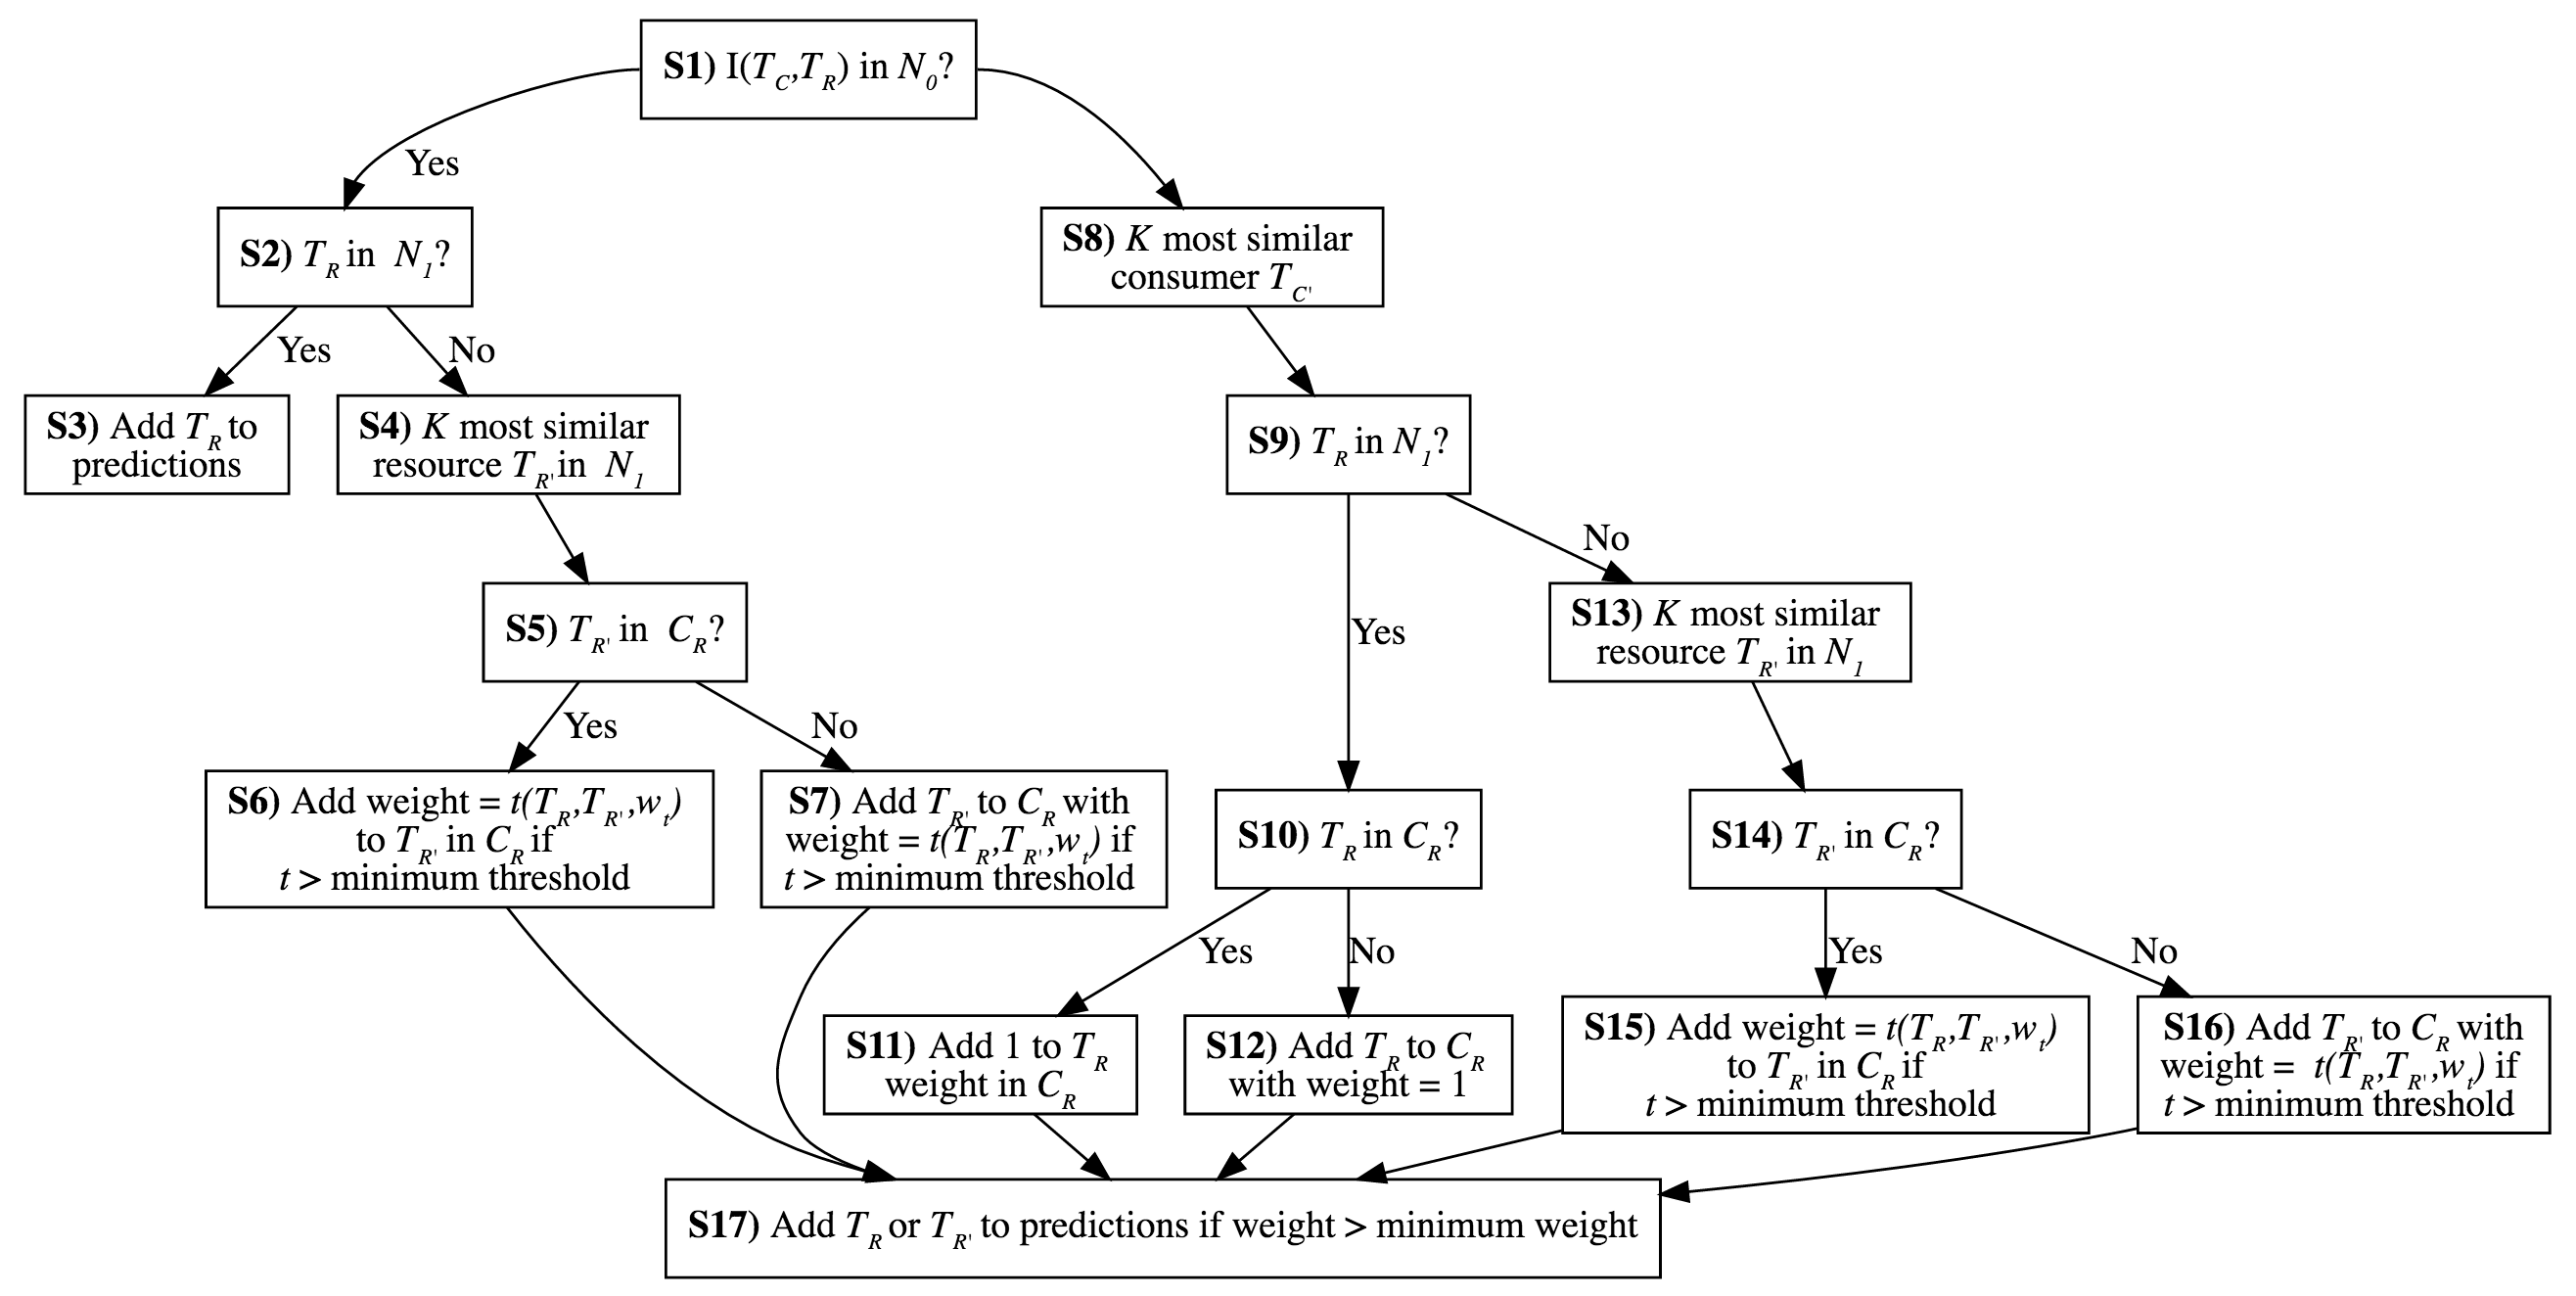
\includegraphics[width=\textwidth]{./chapitre3/figures/Decision_Diagram.png}
      \caption{Description of 17 logical steps (S1-S17) used by the algorithm to suggest a list of candidate resources ($C_R$) for each consumer taxa ($T_C$) in a set of $N_1$ for which interactions are predicted, using a set of taxa $N_0$ with empirically described interactions. Interactions between consumer and resource taxa are denoted as I($T_C$,$T_R$). $K$ is the number of most similar neighbours selected for the KNN algorithm; $t$ stands for tanimoto in equation 1; $w_t$ is the weight given to sets of resources and consumers in equation 2; the minimum threshold is a value setting the minimal similarity value accepted for taxa to be considered as close neighbours in the KNN algorithm; the weight is the value added to a candidate resource each time it is added to $C_R$; the minimum weight is the minimal weight value accepted for candidate resources to be selected as predicted sources in the algorithm.}
      \label{fig:decision_diag}
\end{figure}

% Figure 2
\newpage
    \begin{figure}[h]
      \centering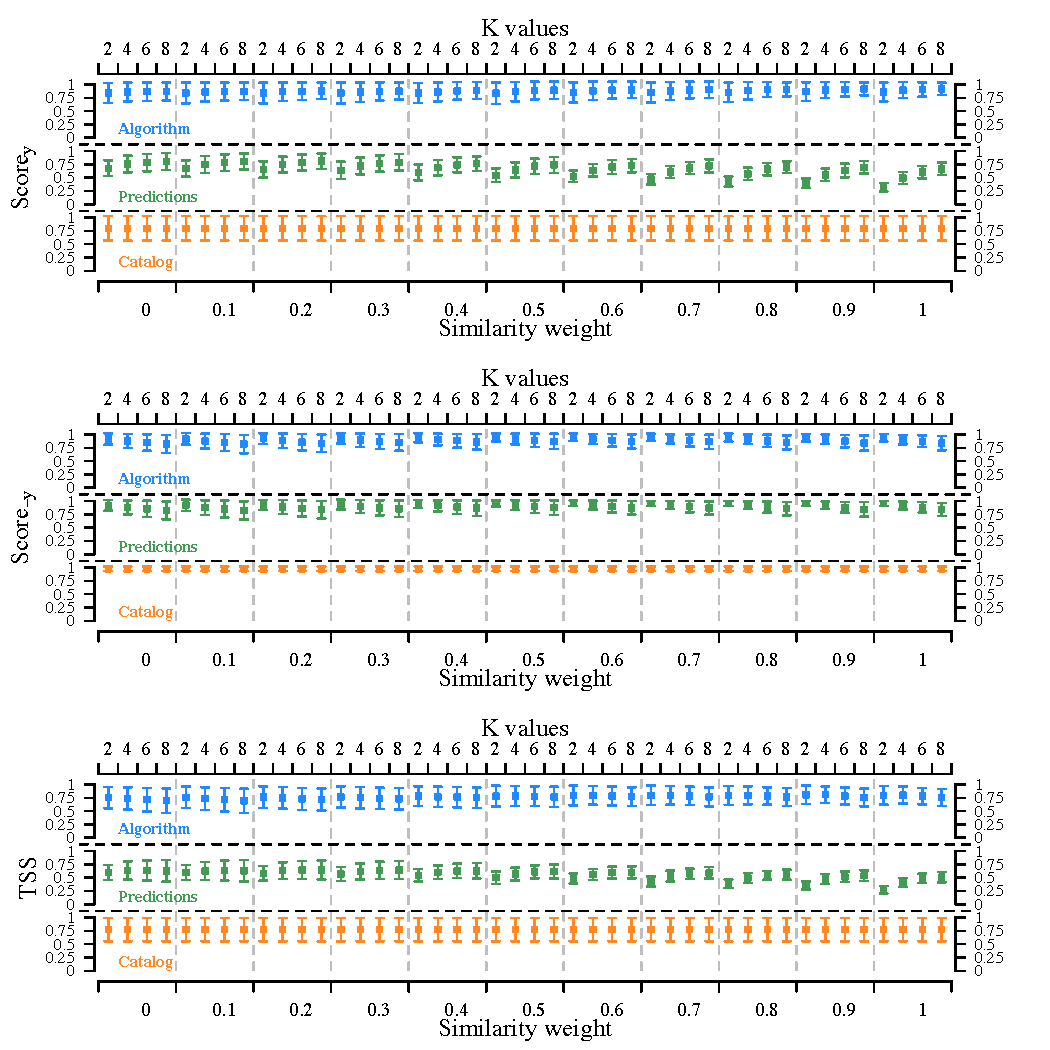
\includegraphics[width=\textwidth, height=12cm]{./chapitre3/figures/multiple_parameters2.pdf}
      \caption{Representation of the three statistics ($i.e.$ $Score_y$, $Score_{\neg y}$ and TSS) used to evaluate the accuracy of the algorithm as a function of $K$ values tested ($i.e.$ 2, 4, 6 and 8 most similar seighbours, top $x$-axis) and weight for taxonomy (bottom $x$-axis), which varies between 0 and 1. A weight of 0 means that similarity is measured only using set of resources/consumers for each taxa, while a weight of 1 means that similarity is based solely on taxonomy. For each statistic, the topmost panel presents prediction accuracy for the complete algorithm, the middle panel corresponds to predictions made through the predictive portion of the algorithm (Steps S4-S16; Figure \ref{fig:decision_diag}) and the bottom panal presents the catalogue contribution for the algorithm (Steps S1-S3; Figure \ref{fig:decision_diag}). Note that the sum of the predictive and catalogue contributions can be over 100\% as there is overlap between predictions made through both. The 7 datasets used for this analysis contained over 50 taxa \citep{christian1999, link2002, brose2005, thompson2004, barnes2008, kortsch2015}}.
      \label{fig:multi_param}
    \end{figure}

% Figure 3
\newpage
    \begin{figure}[h]
      \centering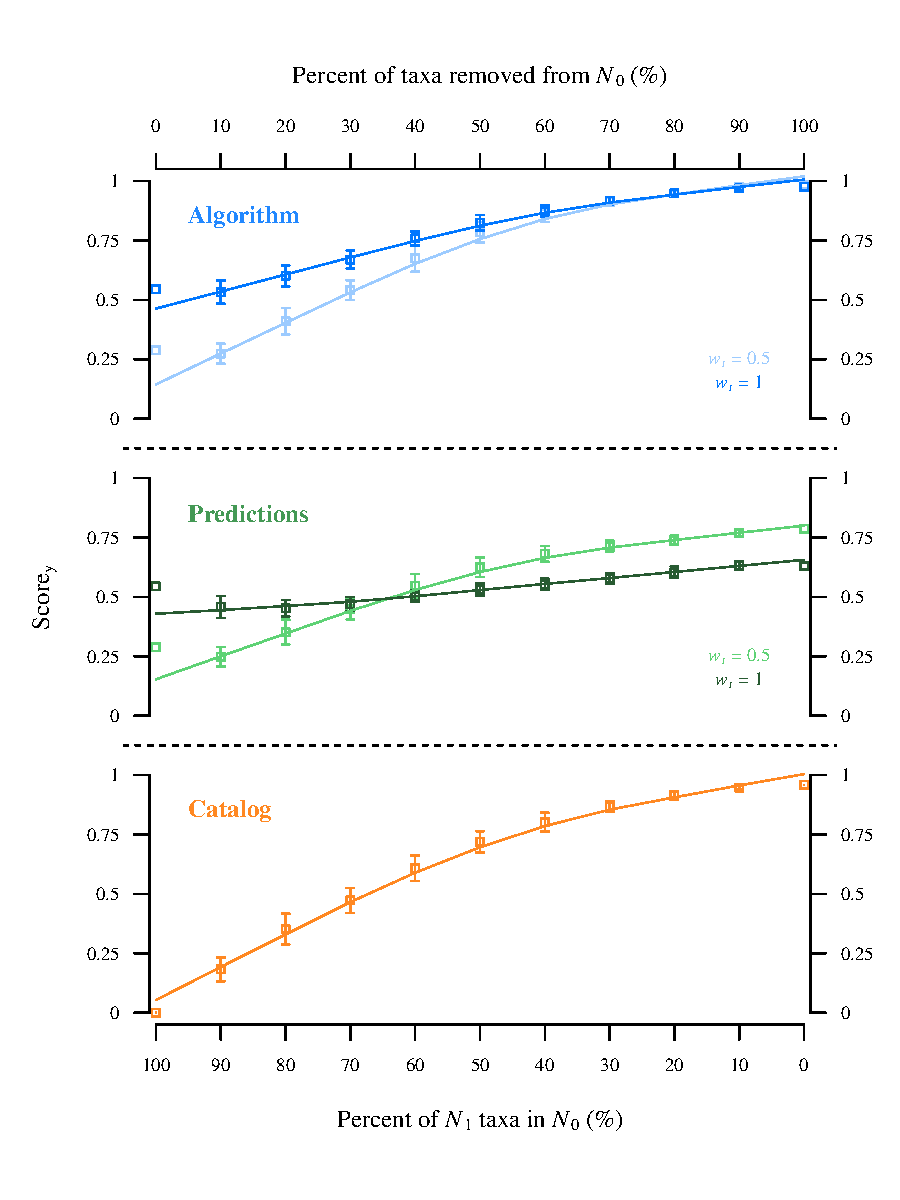
\includegraphics[height=35em]{./chapitre3/figures/catalog_predictions3.pdf}
      % \caption{Caption on next page.}
      \caption{Representation of $Score_y$ as a function of catalogue comprehensiveness, $i.e.$ the amount of information on sets of consumer and resources available in the catalogue. The sensitivity of the algorithm to data accuracy was evaluation with the arctic food web from \citet{kortsch2015}. This food web was highly detailed taxonomically. Once removed from the catalogue, almost 100\% of its taxa still had information available on sets of consumers and resources, which necessary for testing the impact of catalogue comprehensiveness on prediction accuracy. A random percentage of data available in the catalogue for taxa in the food web ($i.e.$ 0 to 100\%) was iteratively removed ($n$ = 50 randomizations) before generating new predictions with the algorithm. $w_t$ values of 0.5 and 1 were evaluated to verify the usefulness of taxonomy in supporting predictive accuracy. The topmost panel presents prediction accuracy for the complete algorithm, the middle panel corresponds to predictions made through the predictive portion of the algorithm (Steps S4-S16; Figure \ref{fig:decision_diag}) and the bottom panel presents the catalogue contribution for the algorithm (Steps S1-S3; Figure \ref{fig:decision_diag}). Note that the sum of the predictive and catalogue contributions can be over 100\% as there is overlap between predictions made through both.}
      \label{fig:catalog_pred}
    \end{figure}

% Figure 4
\newpage
    \begin{figure}[h!]
      \centering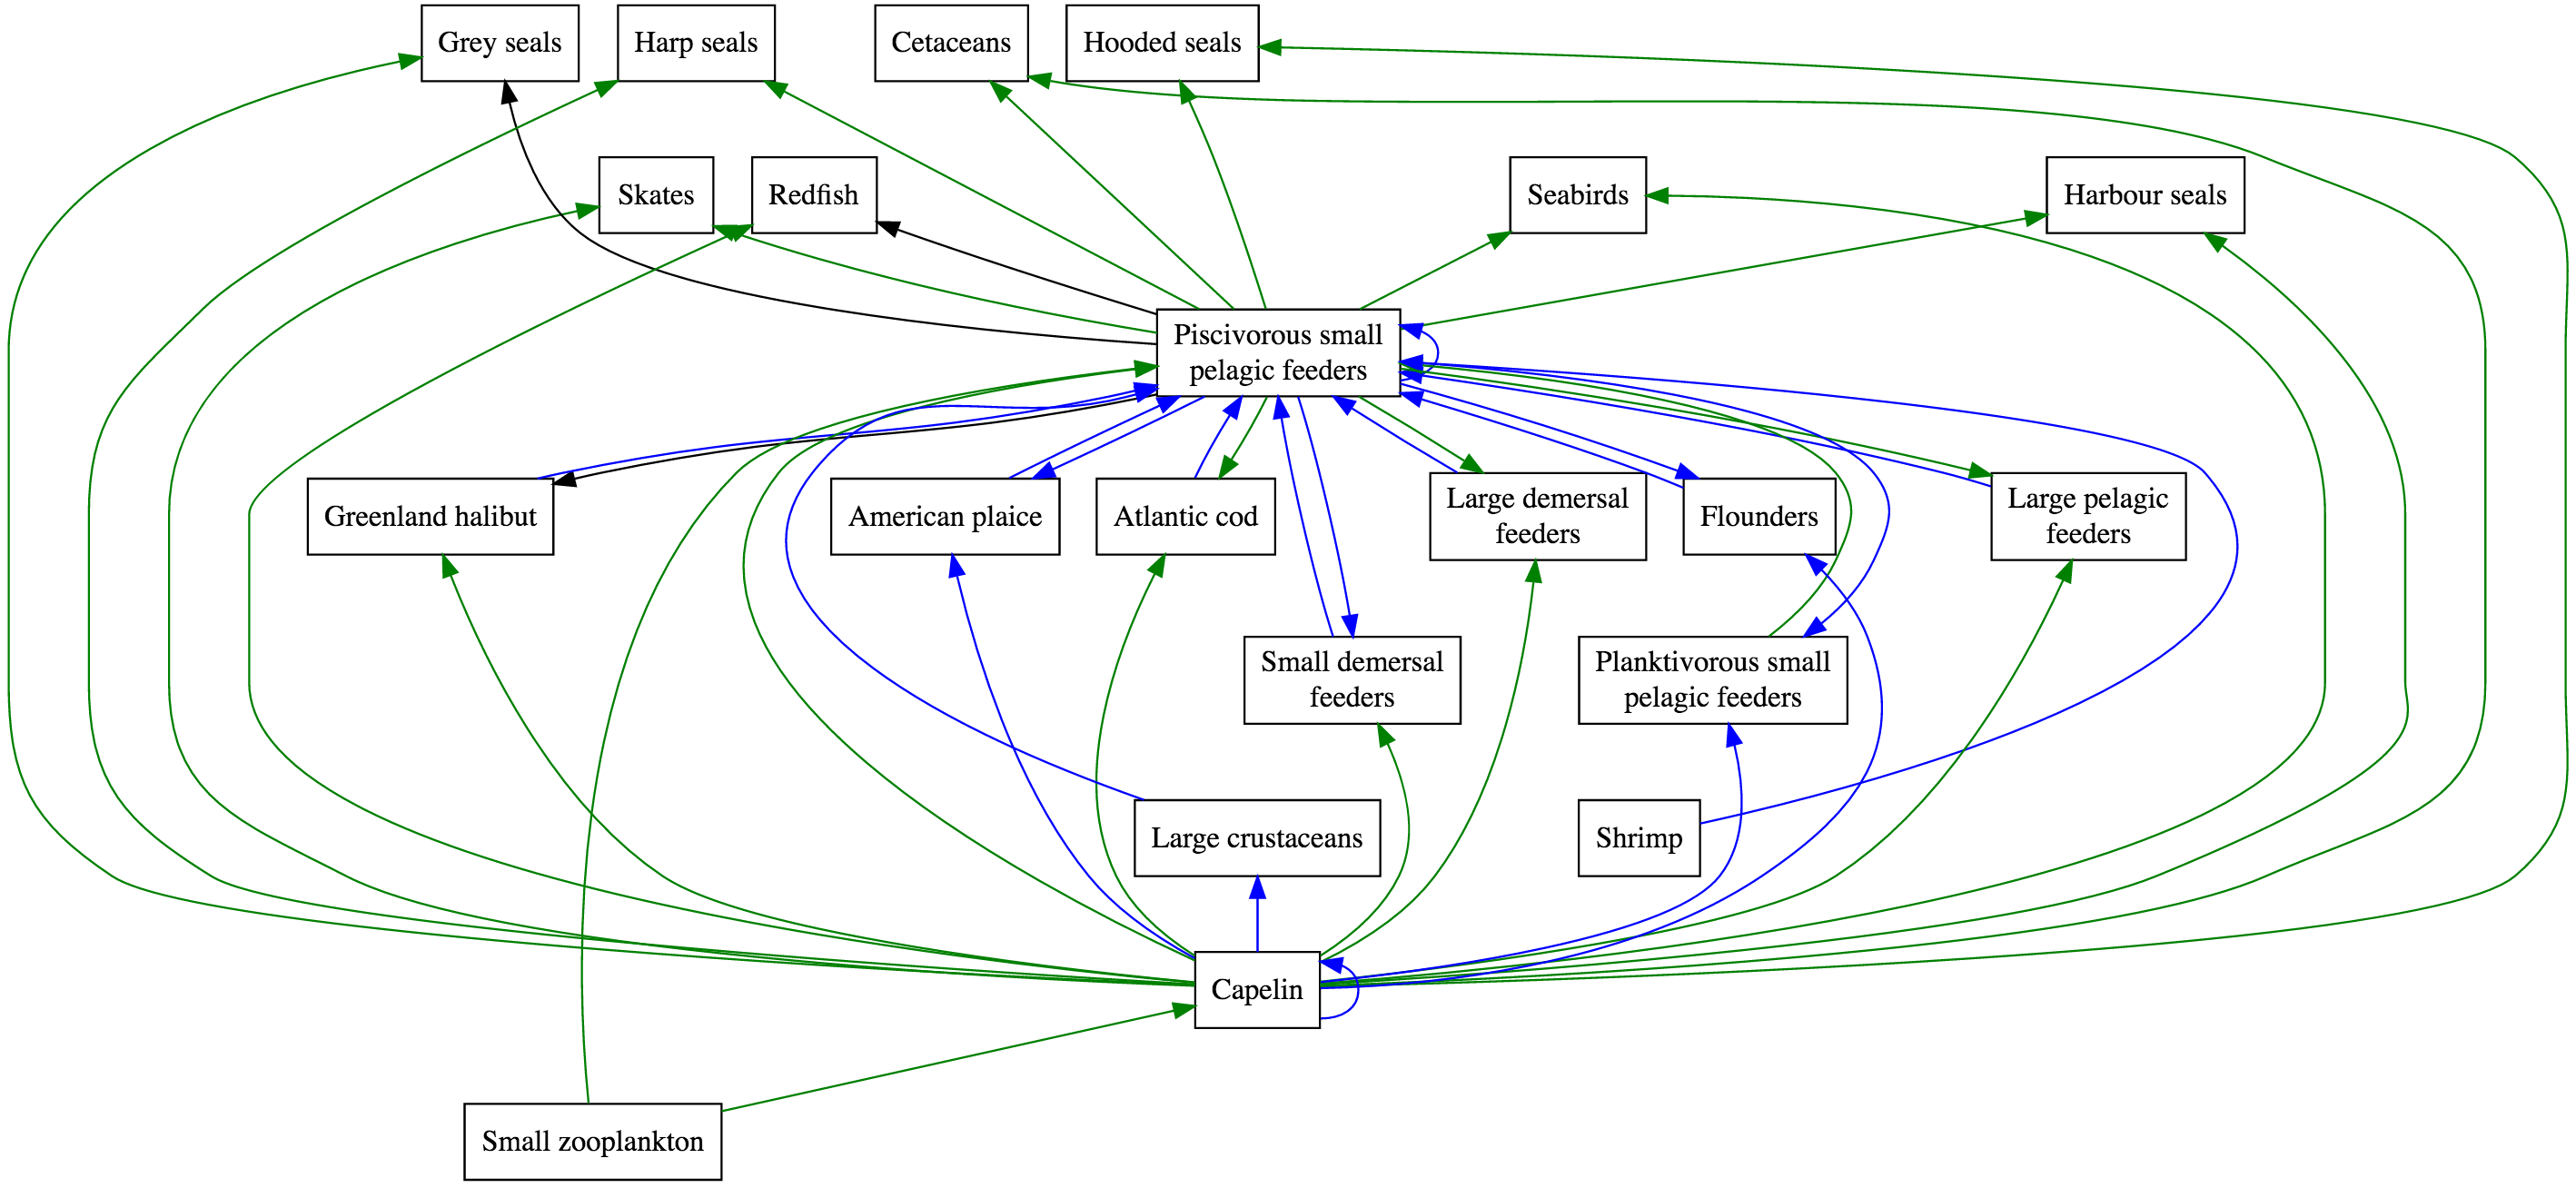
\includegraphics[width=\textwidth]{./chapitre3/figures/SGSL.png}
      \caption{Example of predicted interactions with the network of the southern Gulf of St. Lawrence \citep{savenkoff2004}, centered around the interactions of the capelin (\textit{Mallotus villosus}) and piscivorous small pelagic feeders (\textit{e.g. Scomber scombrus $and$ Illex illecebrosus}). Edge with colors green were both predicted and observed (26), black were observed only (3) and blue were predicted only (19). Arrows are pointed towards consumers.}
      \label{fig:SGSL}
    \end{figure}
